\customchapter{INTRODUCCIÓN} 

\section{Presentación del tema de investigación}

La calidad del entorno en espacios interiores, conocida como Calidad Ambiental Interior (IEQ, por sus siglas en inglés), abarca una diversidad de elementos que influyen en el ambiente, incluyendo el confort térmico, la calidad del aire, las condiciones acústicas y el confort visual, entre otros aspectos como el diseño interior o la ubicación del edificio \cite{source1}. De estos componentes, el confort térmico, la calidad del aire interior (CAI), la acústica y el confort visual son los que se pueden monitorear físicamente y se consideran particularmente relevantes para la salud y productividad de las personas \cite{source1}.

La relevancia de mantener una adecuada calidad del aire interior se justifica dado que la mayoría de las personas pasan alrededor del 90\% de su tiempo en estos ambientes \cite{its_about_time_a_comparison_of_canadian_and_american_time_activity_patterns}. En este contexto, entre los principales enfoques de los sistemas de monitoreo de la calidad de aire en espacios cerrados desde el año 2015 está la medición y seguimiento de los niveles de dióxido de carbono (CO\(_2\)), los cuales se realizan en un 65\% de ellos \cite{IAQ_monitoring_systems_based_on_internet_of_things_a_systematic_review}. El interés por este parámetro se debe a la relación que existe entre los altos niveles de CO\(_2\) y distintos efectos perjudiciales a nivel fisiológico y psicomotor \cite{effects_of_low_level_inhalation_exposure_to_carbon_dioxide_in_indoor_environments_a_short_review_on_human_health_and_psychomotor_performance}.

Debido a esta importancia, tanto organizaciones internacionales como nacionales han emitido regulaciones sobre los niveles de CO\(_2\) en espacios cerrados. La base de datos de la Sociedad Internacional de la Calidad del Aire Interior y Clima (ISIAQ) indica que la moda del valor máximo permitido de CO\(_2\) en interiores es de 1000 ppm, con rangos que varían entre 700 ppm y 1500 ppm \cite{indoor_air_quality_guidelines_from_across_the_world_an_appraisal_considering_energy_saving_health_productivity_and_comfort, ISIAQ_database}. En el ámbito nacional peruano, la directiva administrativa N°349-MINSA/DGIESP-2024 señala que un umbral adecuado de concentración de CO\(_2\) es 400 ppm sobre el nivel de base (ambiente sin personas), y es deseable que no se sobrepasen las 1000 ppm \cite{directiva_minsa}.

Tradicionalmente, la evaluación de la IEQ ha sido una tarea compleja que requería equipos especializados de grado científico y procedimientos de medición detallados \cite{source1}. Sin embargo, la reciente aparición en el mercado de monitores ambientales de bajo costo basados en el Internet de las Cosas (IoT) ha generado un creciente interés en la comunidad científica para evaluar su potencial \cite{source1}. Estos dispositivos, a menudo en un rango de precio de hasta 500 EUR, con la mayoría situándose entre 200 y 350 EUR, prometen una mayor accesibilidad \cite{source1}.

Si bien gran parte de la investigación con estos dispositivos económicos se ha centrado en la calidad del aire interior, especialmente en la detección de partículas, algunos estudios han ampliado el alcance para incluir otros parámetros como el CO\(_2\), compuestos orgánicos volátiles totales (VOCs), temperatura y humedad relativa \cite{source1}. El tema es de particular relevancia en ingeniería debido a la creciente adopción de tecnologías IoT en sectores como el cuidado de la salud y la educación. El IoT constituye soluciones tecnológicas mediante la integración de sensores y otros componentes de hardware en un ecosistema que les permite interactuar para gestionar datos y acciones \cite{the_application_of_internet_of_things_in_healthcare_a_systematic_literature_review_and_classification}. Proyectos que exploran el uso de tecnología IoT para el monitoreo ambiental tanto en interiores como exteriores, utilizando plataformas como Arduino, Raspberry Pi y tecnologías de comunicación como LoRaWAN, han sido desarrollados \cite{source3, source5, source6, source8}, con visualización de datos a través de plataformas IoT especializadas \cite{source3, source5, source8, source12}.

No obstante, el consumo energético es una preocupación principal en aplicaciones de monitoreo en tiempo real, determinado predominantemente por el protocolo de comunicación \cite{IAQ_monitoring_systems_based_on_internet_of_things_a_systematic_review}. Alternativas de bajo consumo como Bluetooth o ZigBee son utilizadas para áreas reducidas debido a limitaciones de alcance. Tecnologías de largo alcance como Wi-Fi pueden no ser deseables para implementaciones como un campus inteligente debido a su alto consumo energético. Para tales aplicaciones, se requiere un protocolo adecuado en términos de consumo y alcance, como LoRa, que cumple estos requerimientos para distancias de pocos kilómetros \cite{source3, source5, source9, source10}.

Un enfoque holístico para la evaluación de la IEQ es fundamental para entender la interacción entre sus diversos componentes y para desarrollar un índice unificado de IEQ, que incluya coeficientes de ponderación que reflejen la importancia mutua de estos factores \cite{source1}. Este proyecto de investigación se enmarca en este contexto, buscando desarrollar un índice de IEQ y un prototipo de sistema de monitoreo IoT accesible y funcional, utilizando tecnología LoRa, para evaluar la calidad ambiental en espacios cerrados dentro de un campus universitario.























\section{Descripción de la situación problemática}

A pesar del reconocimiento de la importancia de la Calidad Ambiental Interior (IEQ) para la salud y la productividad \cite{source1}, su monitoreo tradicional ha sido costoso y poco accesible para el usuario común debido al uso de equipos especializados y procedimientos complejos \cite{source1}. La aparición de monitores IoT de bajo costo ha comenzado a cambiar este panorama, democratizando la posibilidad de medir parámetros ambientales \cite{source1}. Tras la pandemia de SARS-CoV-2, que reveló vulnerabilidades y la falta de controles adecuados, el monitoreo de los niveles de CO\(_2\) ha adquirido una relevancia aún mayor, no solo por sus efectos adversos, sino también porque es un indicador clave del riesgo de contagio en ambientes cerrados.

Sin embargo, la mayoría de las evaluaciones y el desarrollo de estos dispositivos económicos se han centrado principalmente en componentes individuales de la IEQ, como la calidad del aire interior, a menudo limitándose al monitoreo de partículas o dióxido de carbono \cite{source1}. Actualmente, no existe en el mercado un monitor de grado de consumo que ofrezca una evaluación holística de la IEQ, integrando mediciones de diversos parámetros ambientales de manera comprensiva \cite{source1}.

Muchos de los proyectos de monitoreo de IEQ con dispositivos de bajo costo, como los basados en Arduino, se encuentran en etapas de prueba de concepto, y su rendimiento y fiabilidad en despliegues reales a gran escala aún no están completamente documentados o garantizados \cite{source1}. La necesidad de medir la IEQ de manera integral es crucial para poder caracterizar la importancia de sus componentes e integrar esta información en un índice unificado que sea fácil de interpretar \cite{source1}.

Específicamente en entornos educativos como las universidades, mantener una buena calidad ambiental interior es un desafío relevante. Estudios sobre la calidad del aire en salones universitarios han identificado espacios con concentraciones de CO\(_2\) que superan los límites admisibles, lo que puede generar malestar físico en los estudiantes y aumentar el riesgo de transmisión de virus \cite{source23}. Aunque se han implementado sistemas de monitoreo, la cobertura total de los espacios, la integración de diversas variables ambientales más allá del CO\(_2\), y el uso de equipos con alta precisión o capacidades avanzadas de análisis pueden requerir una inversión significativa \cite{source23, source24}. La facilidad de uso y la accesibilidad de la información para los ocupantes finales también son aspectos a mejorar en los sistemas existentes \cite{source1}.

En este contexto, la situación problemática se centra en la brecha existente entre la necesidad de un monitoreo integral y accesible de la IEQ en espacios universitarios y la disponibilidad actual de soluciones tecnológicas que sean a la vez de bajo costo, holísticas, fáciles de usar e implementar.








\introsection{Formulación del problema}

%El presente proyecto se centra en el diseño e implementación de una alternativa de robot de vigilancia y patrullaje capaz de identificar intrusos mediante procesamiento de imágenes. Para ello se escogió un robot de dos ruedas de tipo péndulo invertido, pues permite operar con mayor facilidad en espacios estrechos, y hacerlo con mayor rapidez que un robot de cuatro ruedas, lo que le permite adaptarse mejor a la estructura de las instalaciones en las que será usado \cite{TWR_advantages}. Para controlar el robot, se seleccionó el controlador adaptativo por modelo de referencia directo (MRAC directo) debido a que es un algoritmo de control robusto que permite controlar el robot sobre distintas superficies. Con respecto a los algoritmos de procesamiento de imágenes para patrullaje y detección de intrusos se seleccionó el clasificador Haar Cascade para detección de personas y el algoritmo de localización y el algoritmo de localización y mapeo simultáneos (SLAM) para ubicar el lugar las detecciones en el mapa de las instalaciones. Para incrementar la tasa de cuadros por segundo procesados, se implementó parte de los algoritmos de procesamiento de imágenes en lógica programable, es decir, circuitos lógicos secuenciales reconfigurables, como los FPGA (Field-Programmable Gate Arrays).

Dado el impacto de los altos niveles de CO\(_2\) en la salud y el rendimiento académico, especialmente en entornos cerrados como aulas, surge la pregunta: ¿Cómo podemos diseñar e implementar un sistema de monitoreo basado en IoT que mida, registre y alerte sobre los niveles de CO\(_2\) en tiempo real, asegurando que los ambientes educativos se mantengan dentro de los límites saludables establecidos?


\introsection{Objetivos de investigación}
En esta sección se presentan los objetivos de este Trabajo Final de Ingeniería Mecatrónica. Sobre ellos se estructuró la investigación y los resultados presentados.

\subsubsection*{Objetivo general}
Desarrollar un Índice de Calidad Ambiental Interior (IEQ) e implementar un prototipo funcional de sistema de monitoreo IoT basado en LoRa, compuesto por tres nodos sensores, para la evaluación y visualización de la calidad ambiental en espacios cerrados dentro de un campus universitario.

\subsection*{Objetivos Específicos}

\begin{itemize}
    \item Analizar la literatura científica y normativa referente a los parámetros clave de la calidad ambiental interior (CO\(_2\), material particulado PM\textsubscript{2.5}, temperatura y humedad), incluyendo sus umbrales de referencia y las metodologías existentes para la formulación de índices de calidad ambiental.
    \item Establecer sub-índices para los parámetros ambientales seleccionados (CO\(_2\), PM\textsubscript{2.5}, temperatura y humedad), determinando rangos y sistemas de puntuación fundamentados en la literatura científica para categorizar los niveles de calidad o confort.
    \item Desarrollar una metodología de ponderación y agregación, claramente justificada, para los sub-índices definidos, orientada a la obtención de un Índice de Calidad Ambiental Interior (IEQ) unificado, simplificado y de fácil interpretación.
    \item Diseñar la arquitectura e implementar un prototipo funcional de un sistema de monitoreo ambiental IoT, empleando tecnología LoRa para la comunicación inalámbrica de datos desde tres nodos sensores (para la medición de CO\(_2\), PM\textsubscript{2.5}, temperatura y humedad) hacia un dispositivo gateway.
    \item Configurar la transmisión de datos desde los nodos sensores hacia el gateway y, subsecuentemente, a una plataforma en la nube para su almacenamiento básico y visualización.
    \item Incorporar el IEQ formulado en la plataforma de visualización del prototipo, habilitando la observación en tiempo real del índice calculado a partir de los datos adquiridos por los sensores.
    \item Ejecutar pruebas funcionales del prototipo implementado para validar la correcta recolección, transmisión, almacenamiento y visualización de datos, así como el cálculo del IEQ, en espacios seleccionados del campus universitario.
    \item Elaborar la documentación técnica detallada del diseño del IEQ, su fundamentación teórica, la arquitectura e implementación del prototipo del sistema de monitoreo IoT-LoRa (incluyendo nodos y gateway), los resultados de las pruebas funcionales, y las consideraciones para su aplicabilidad y potencial escalabilidad en un entorno universitario.
\end{itemize}


\introsection{Justificación}

%Desarrollar este proyecto permite contar con una alternativa de robot de patrullaje y vigilancia capaz de ejecutar el algoritmo de detección de intrusos en el mismo robot a una mayor tasa de cuadros por segundo gracias a la aceleración por hardware. Esta alternativa resulta particularmente útil para casos en los que el territorio extenso, no se cuenta con una red WI-FI local a la cual conectarse para hacer el procesamiento de imágenes en una computadora física y no es viable instalar un router portátil en el robot debido a que no hay cobertura de servicios de internet, como en zonas rurales, o no se desea enviar los datos a la nube para su procesamiento.

La calidad del aire en espacios cerrados ha adquirido gran importancia en los últimos años debido a los riesgos que altos niveles de CO\(_2\) representan para la salud humana y la productividad. Estudios recientes han demostrado que concentraciones elevadas de CO\(_2\) en interiores no solo afectan el rendimiento cognitivo y físico, sino que también son un indicador clave del riesgo de contagio y proliferación de microorganismos, un aspecto que ha cobrado relevancia tras la pandemia de SARS-CoV-2.

En el ámbito educativo, donde estudiantes y docentes pasan la mayor parte del tiempo en salones de clase, es esencial garantizar una adecuada calidad del aire. Sin embargo, muchos centros educativos no cuentan con sistemas de monitoreo que permitan medir en tiempo real los niveles de CO\(_2\), lo que puede derivar en ambientes no saludables que impactan negativamente tanto en el bienestar como en el rendimiento académico.

A pesar de los avances en tecnología IoT, la implementación de redes de monitoreo eficientes sigue siendo un reto. Este proyecto se enfoca en diseñar e implementar una red IoT de nodos sensores para medir los niveles de CO\(_2\) en aulas, recopilando esta información en una base de datos en la nube. El objetivo es poder alertar de manera oportuna cuando se sobrepasen los límites de CO\(_2\) permitidos, asegurando que el ambiente sea siempre apto para las personas, y así contribuir a la creación de entornos educativos más seguros y saludables, en línea con las regulaciones nacionales e internacionales vigentes sobre calidad del aire en interiores.


\subsection*{Alcances y Limitaciones}

El alcance del proyecto comprende el diseño teórico del Índice de Calidad Ambiental Interior (IEQ) y la implementación de un prototipo funcional del sistema de monitoreo IoT-LoRa. Se definirán los parámetros del IEQ (CO\(_2\), PM\textsubscript{2.5}, temperatura y humedad), sus rangos y la metodología de cálculo basada en la revisión de literatura científica y estándares existentes. Asimismo, se implementará un prototipo con tres nodos sensores que medirán los parámetros definidos, utilizando tecnología LoRa para la comunicación inalámbrica con un gateway, y se configurará la transmisión de datos desde los nodos al gateway y de este a una plataforma en la nube para su almacenamiento básico y visualización, donde se mostrará el IEQ calculado. Las pruebas funcionales del prototipo se realizarán en un número limitado de espacios cerrados dentro del campus universitario para demostrar su operatividad. Es importante destacar que no se contempla la construcción de carcasas o gabinetes protectores para los nodos sensores ni para el gateway del prototipo, y la validación del IEQ se basará en su fundamentación teórica y en la coherencia de los resultados del prototipo durante las pruebas funcionales, sin incluir estudios de percepción de confort con ocupantes.

Las limitaciones del proyecto incluyen principalmente el factor tiempo, ya que el desarrollo está restringido a un periodo de 7 semanas, lo que condiciona la profundidad de la experimentación, el número de nodos a implementar y la exhaustividad de las pruebas. Adicionalmente, un presupuesto limitado restringe la cantidad y tipo de sensores, fijando el número de nodos sensores en tres para este prototipo, así como la sofisticación de los componentes del gateway y la plataforma de visualización. La implementación física se materializará en un prototipo funcional básico, sin contemplar un despliegue a gran escala ni una optimización para producción masiva; la robustez del hardware estará, por tanto, sujeta a los componentes de bajo costo disponibles y no se diseñarán ni construirán carcasas o gabinetes protectores, lo que podría limitar su durabilidad y protección a largo plazo. En cuanto a la validación del Índice IEQ, esta se limitará a los datos recolectados por el prototipo durante las pruebas funcionales, sin realizar estudios comparativos con equipos de referencia de alta precisión ni encuestas detalladas de percepción de confort a los ocupantes. La definición de umbrales y, especialmente, las ponderaciones para los parámetros del IEQ dependerán de la información disponible y consensuada en la literatura científica. Finalmente, las pruebas funcionales del prototipo se realizarán en un número limitado de espacios dentro del campus universitario, por lo que los resultados podrían no ser generalizables a todos los tipos de recintos sin adaptaciones, y no se realizarán estudios exhaustivos de cobertura de la señal LoRa en todo el campus ni análisis detallados de interferencias.

d

\introsection{Organización del trabajo de investigación}
El plan de trabajo de esta investigación se muestra en la tabla \ref{tab: gantt}.

\begin{table}[H]
\centering
    \caption{\centering Diagrama de Gantt del proyecto.}
    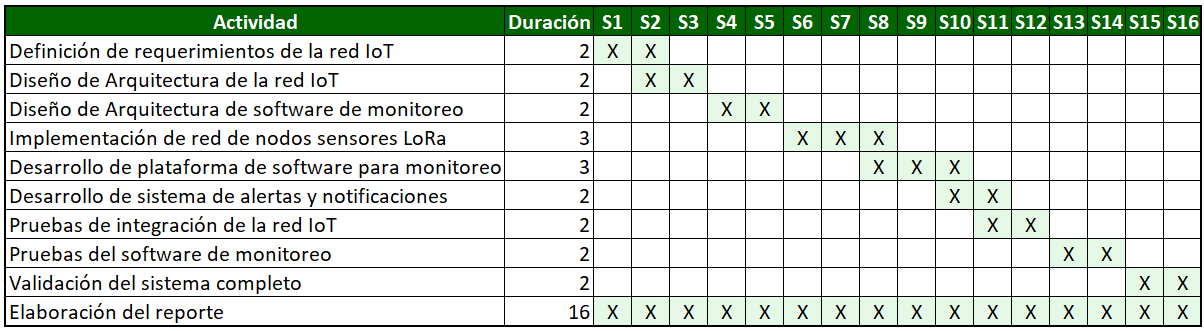
\includegraphics[width=1\linewidth]{images/Introduccion/Gantt.png}
\label{tab: gantt}
\end{table}

Este trabajo de investigación está organizado de la siguiente forma. El Capítulo I, la revisión de la literatura, presenta sistemas de medición y monitoreo de CO\(_2\) en espacios cerrados en proyectos de investigación como estado del arte e investigaciones relacionadas a herramientas de monitoreo manuales de CO\(_2\) u otros sistemas de medición de gases en espacios cerrados como trabajos previos. En el capítulo II, el marco teórico, se presenta tanto la arquitectura de la red IoT que contiene los nodos sensores, así como la arquitectura de software que se utilizará para el programa de monitoreo. En el Capítulo III, el marco metodológico, se presenta la implementación de red de nodos sensores LoRa, el desarrollo de la plataforma de software de monitoreo y el sistema de alertas y notificaciones. En el Capítulo IV, de resultados, se presentan las pruebas de integración de la red IoT, las pruebas del software de monitoreo y el sistema de alertas, y la validación del sistema completo. Por último, se abordan las conclusiones en relación con los objetivos planteados y se hacen recomendaciones para trabajos futuros.
